% Source: TeX Live 2025 PGF manual, pgfmanual-en-library-lsystems.tex
\documentclass[border=2pt]{standalone}
\usepackage{tikz}
\usetikzlibrary{lindenmayersystems}

\begin{document}
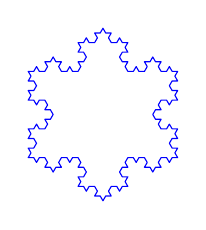
\begin{tikzpicture}
\pgfdeclarelindenmayersystem{Koch curve}{
  \rule{F -> F-F++F-F}
}
\draw[blue, line join=round]
  [l-system={Koch curve, step=2pt, angle=60, axiom=F++F++F, order=3}]
  lindenmayer system -- cycle;
\end{tikzpicture}
\end{document}
